
\documentclass[10 pt,usenames,dvipsnames, oneside]{article}
\usepackage{../../modelo-fracoes}
\graphicspath{{../../../Figuras/licao04/}}


\begin{document}

\begin{center}
  \begin{minipage}[l]{3cm}

\includegraphics[width=2cm]{../../../Figuras/logo}       
\end{minipage}\hfill
\begin{minipage}[r]{.8\textwidth}
 {\Large \scshape Atividade: Oito panquecas para 24 amigos}  
\end{minipage}
\end{center}
\vspace{.2cm}

\ifdefined\prof
%Caixa do Para o Professor
\begin{goals}
%Objetivos específicos
\begin{enumerate}
\item       Obter uma fração irredutível equivalente a uma fração dada e
relacionar esta equivalência no contexto de minimização de cortes em uma
equipartição.
\end{enumerate}

\tcblower

%Orientações e sugestões
\begin{itemize}
\item       Recomenda-se que, nesta atividade, os alunos trabalhem
individualmente ou em duplas. No entanto, é fundamental que os alunos sejam
estimulados a explicar o raciocínio realizado.
\item       A discussão da atividade, além da equipartição dada e aquela
associada ao número mínimo de cortes, pode incluir as equipartições associadas a
outras frações equivalentes a       $\dfrac{8}{24}$      :       $\dfrac{4}{12}$
(divisão de cada panqueca em 12 partes iguais) e       $\dfrac{2}{6}$
(divisão da panqueca em 6 partes iguais).
\end{itemize}
\end{goals}

\bigskip
\begin{center}
{\large \scshape Atividade}
\end{center}
\fi

\textit{(Adaptado de Empson (2001))}

$24$ amigos estão querendo dividir igualmente $8$ panquecas circulares.

Luciano, um dos amigos sugeriu que cada panqueca fosse dividida em $24$ partes iguais e que, então, cada um dos 24 amigos recebesse $8$ dessas partes.
\begin{center}
 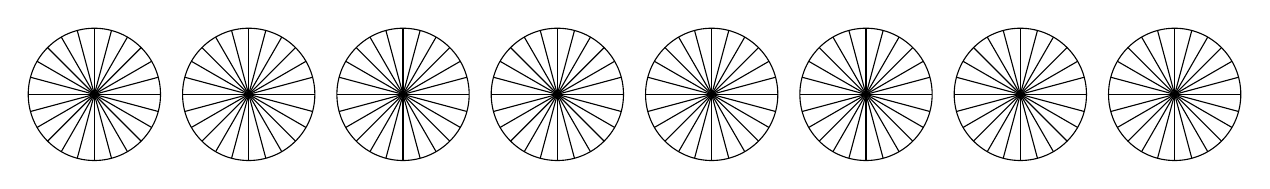
\begin{tikzpicture}[x=0.2cm,y=0.2cm, scale=1.4]
%\clip(-6.671687478832792,-17.90763699164108) rectangle (54.671411657651255,12.538800286189925);
\draw(0.,0.) circle (0.6cm);
\draw(7.,0.) circle (0.6cm);
\draw(14.,0.) circle (0.6cm);
\draw(21.,0.) circle (0.6cm);
\draw(28.,0.) circle (0.6cm);
\draw(35.,0.) circle (0.6cm);
\draw(42.,0.) circle (0.6cm);
\draw(49.,0.) circle (0.6cm);
\draw (0.,0.)-- (3.,0.);
\draw (0.,0.)-- (2.897777478867205,0.7764571353075622);
\draw (0.,0.)-- (2.598076211353316,1.5);
\draw (0.,0.)-- (2.121320343559643,2.121320343559643);
\draw (0.,0.)-- (1.5,2.5980762113533165);
\draw (0.,0.)-- (0.7764571353075628,2.8977774788672055);
\draw (0.,0.)-- (0.,3.);
\draw (0.,0.)-- (-0.776457135307562,2.8977774788672055);
\draw (0.,0.)-- (-1.5,2.5980762113533165);
\draw (0.,0.)-- (-2.121320343559643,2.1213203435596433);
\draw (0.,0.)-- (-2.5980762113533165,1.5);
\draw (0.,0.)-- (-2.897777478867206,0.7764571353075632);
\draw (0.,0.)-- (-3.,0.);
\draw (0.,0.)-- (-2.8977774788672064,-0.7764571353075619);
\draw (0.,0.)-- (-2.5980762113533173,-1.5);
\draw (0.,0.)-- (-2.121320343559644,-2.121320343559643);
\draw (0.,0.)-- (-1.5,-2.598076211353317);
\draw (0.,0.)-- (-0.7764571353075636,-2.8977774788672064);
\draw (0.,0.)-- (0.,-3.);
\draw (0.,0.)-- (0.7764571353075618,-2.8977774788672073);
\draw (0.,0.)-- (1.5,-2.5980762113533182);
\draw (0.,0.)-- (2.1213203435596433,-2.121320343559645);
\draw (0.,0.)-- (2.5980762113533173,-1.5);
\draw (0.,0.)-- (2.897777478867207,-0.7764571353075641);
\draw (4.,0.)-- (7.,0.);
\draw (4.102222521132795,0.7764571353075647)-- (7.,0.);
\draw (4.401923788646685,1.5)-- (7.,0.);
\draw (4.878679656440359,2.1213203435596446)-- (7.,0.);
\draw (5.5,2.5980762113533173)-- (7.,0.);
\draw (7.,0.)-- (6.22354286469244,2.897777478867206);
\draw (7.,0.)-- (7.,3.);
\draw (7.,0.)-- (7.776457135307564,2.8977774788672046);
\draw (7.,0.)-- (8.5,2.598076211353315);
\draw (7.,0.)-- (9.121320343559644,2.121320343559641);
\draw (7.,0.)-- (9.598076211353316,1.5);
\draw (7.,0.)-- (9.897777478867205,0.776457135307561);
\draw (7.,0.)-- (10.,0.);
\draw (7.,0.)-- (9.897777478867205,-0.7764571353075636);
\draw (7.,0.)-- (9.598076211353316,-1.5);
\draw (7.,0.)-- (9.121320343559642,-2.1213203435596433);
\draw (7.,0.)-- (8.5,-2.5980762113533165);
\draw (7.,0.)-- (7.776457135307562,-2.8977774788672055);
\draw (7.,0.)-- (7.,-3.);
\draw (7.,0.)-- (6.223542864692438,-2.8977774788672055);
\draw (7.,0.)-- (5.5,-2.5980762113533165);
\draw (7.,0.)-- (4.878679656440357,-2.121320343559643);
\draw (7.,0.)-- (4.401923788646684,-1.5);
\draw (7.,0.)-- (4.102222521132795,-0.7764571353075622);
\draw (14.,0.)-- (11.,0.);
\draw (14.,0.)-- (11.102222521132795,-0.7764571353075622);
\draw (14.,0.)-- (11.401923788646684,-1.5);
\draw (14.,0.)-- (11.878679656440358,-2.121320343559643);
\draw (14.,0.)-- (12.5,-2.598076211353316);
\draw (14.,0.)-- (13.223542864692437,-2.897777478867205);
\draw (14.,0.)-- (14.,-3.);
\draw (14.,0.)-- (14.776457135307563,-2.897777478867205);
\draw (14.,0.)-- (15.5,-2.598076211353316);
\draw (14.,0.)-- (16.121320343559642,-2.121320343559643);
\draw (14.,0.)-- (16.598076211353316,-1.5);
\draw (14.,0.)-- (16.897777478867205,-0.7764571353075631);
\draw (14.,0.)-- (17.,0.);
\draw (14.,0.)-- (16.897777478867205,0.7764571353075614);
\draw (14.,0.)-- (16.598076211353316,1.5);
\draw (14.,0.)-- (16.121320343559642,2.121320343559642);
\draw (14.,0.)-- (15.5,2.598076211353315);
\draw (14.,0.)-- (14.776457135307563,2.897777478867204);
\draw (14.,0.)-- (14.,3.);
\draw (14.,0.)-- (13.223542864692439,2.8977774788672055);
\draw (14.,0.)-- (12.5,2.598076211353317);
\draw (14.,0.)-- (11.878679656440358,2.1213203435596437);
\draw (14.,0.)-- (11.401923788646684,1.5);
\draw (14.,0.)-- (11.102222521132795,0.776457135307564);
\draw (18.,0.)-- (24.,0.);
\draw (18.102222521132795,-0.7764571353075622)-- (23.897777478867205,0.7764571353075614);
\draw (18.401923788646684,-1.5)-- (23.598076211353316,1.5);
\draw (18.878679656440358,-2.121320343559643)-- (23.121320343559642,2.121320343559642);
\draw (19.5,-2.598076211353316)-- (22.5,2.598076211353315);
\draw (20.223542864692437,-2.897777478867205)-- (21.776457135307563,2.897777478867204);
\draw (21.,-3.)-- (21.,3.);
\draw (21.776457135307563,-2.897777478867205)-- (20.223542864692437,2.897777478867205);
\draw (22.5,-2.598076211353316)-- (19.5,2.598076211353316);
\draw (23.121320343559642,-2.121320343559643)-- (18.878679656440358,2.121320343559643);
\draw (23.598076211353316,-1.5)-- (18.401923788646684,1.5);
\draw (23.897777478867205,-0.7764571353075631)-- (18.102222521132795,0.7764571353075631);
\draw (25.,0.)-- (31.,0.);
\draw (25.102222521132795,-0.7764571353075622)-- (30.897777478867205,0.7764571353075614);
\draw (25.401923788646684,-1.5)-- (30.598076211353316,1.5);
\draw (25.878679656440358,-2.121320343559643)-- (30.121320343559642,2.121320343559642);
\draw (26.5,-2.598076211353316)-- (29.5,2.598076211353315);
\draw (27.223542864692437,-2.897777478867205)-- (28.776457135307563,2.897777478867204);
\draw (28.,-3.)-- (28.,3.);
\draw (28.776457135307563,-2.897777478867205)-- (27.223542864692437,2.897777478867205);
\draw (29.5,-2.598076211353316)-- (26.5,2.598076211353316);
\draw (30.121320343559642,-2.121320343559643)-- (25.878679656440358,2.121320343559643);
\draw (30.598076211353316,-1.5)-- (25.401923788646684,1.5);
\draw (25.102222521132795,0.7764571353075631)-- (30.897777478867205,-0.7764571353075631);
\draw (32.,0.)-- (38.,0.);
\draw (32.102222521132795,-0.7764571353075622)-- (37.897777478867205,0.7764571353075614);
\draw (32.401923788646684,-1.5)-- (37.598076211353316,1.5);
\draw (32.878679656440355,-2.121320343559643)-- (37.121320343559645,2.121320343559642);
\draw (33.5,-2.598076211353317)-- (36.5,2.598076211353316);
\draw (34.22354286469244,-2.897777478867206)-- (35.77645713530756,2.897777478867205);
\draw (35.,-3.)-- (35.,3.);
\draw (35.77645713530756,-2.897777478867205)-- (34.22354286469244,2.897777478867204);
\draw (36.5,-2.598076211353317)-- (33.5,2.5980762113533165);
\draw (37.121320343559645,-2.1213203435596437)-- (32.878679656440355,2.1213203435596433);
\draw (37.598076211353316,-1.5)-- (32.401923788646684,1.5);
\draw (37.897777478867205,-0.7764571353075631)-- (32.102222521132795,0.7764571353075627);
\draw (39.,0.)-- (45.,0.);
\draw (39.102222521132795,-0.7764571353075622)-- (44.897777478867205,0.7764571353075614);
\draw (39.401923788646684,-1.5)-- (44.598076211353316,1.5);
\draw (39.878679656440355,-2.121320343559643)-- (44.121320343559645,2.121320343559642);
\draw (40.5,-2.598076211353317)-- (43.5,2.598076211353316);
\draw (41.22354286469244,-2.897777478867206)-- (42.77645713530756,2.897777478867205);
\draw (42.,-3.)-- (42.,3.);
\draw (42.77645713530756,-2.897777478867205)-- (41.22354286469244,2.897777478867204);
\draw (43.5,-2.598076211353317)-- (40.5,2.5980762113533165);
\draw (44.121320343559645,-2.1213203435596437)-- (39.878679656440355,2.1213203435596433);
\draw (44.598076211353316,-1.5)-- (39.401923788646684,1.5);
\draw (44.897777478867205,-0.7764571353075631)-- (39.102222521132795,0.7764571353075627);
\draw (46.,0.)-- (52.,0.);
\draw (46.102222521132795,-0.7764571353075622)-- (51.897777478867205,0.7764571353075614);
\draw (46.401923788646684,-1.5)-- (51.598076211353316,1.5);
\draw (46.878679656440355,-2.121320343559643)-- (51.121320343559645,2.121320343559642);
\draw (47.5,-2.598076211353317)-- (50.5,2.598076211353316);
\draw (48.22354286469244,-2.897777478867206)-- (49.77645713530756,2.897777478867205);
\draw (49.,-3.)-- (49.,3.);
\draw (49.77645713530756,-2.897777478867205)-- (48.22354286469244,2.897777478867204);
\draw (50.5,-2.598076211353317)-- (47.5,2.5980762113533165);
\draw (51.121320343559645,-2.1213203435596437)-- (46.878679656440355,2.1213203435596433);
\draw (51.598076211353316,-1.5)-- (46.401923788646684,1.5);
\draw (51.897777478867205,-0.7764571353075631)-- (46.102222521132795,0.7764571353075627);
\end{tikzpicture}
\end{center}

\begin{enumerate} %d
  \item     Com a divisão sugerida por Luciano, qual a fração de uma panqueca que cada amigo vai receber?
  \item     Quantos cortes da panqueca (do centro para a borda, como no desenho) são necessários para a divisão proposta?
  \item     É possível dividir igualmente as     $8$ panquecas entre os     $24$ amigos fazendo menos cortes do que como Luciano sugeriu? Se você acha que sim, quantos cortes serão necessários e qual é a fração de uma panqueca que cada amigo poderia receber neste caso?
\end{enumerate} %d

\ifdefined\prof
\begin{solucao}

\begin{enumerate}
\item       Cada amigo vai receber       $\dfrac{8}{24}$       de panqueca.
\item             $8 \times 24 = 192$       cortes.
\item       Sim! Por exemplo, como       $\dfrac{8}{24} = \dfrac{8 \times 1}{8
\times 3} = \dfrac{1}{3}$, basta dividir cada panqueca       $3$       partes
iguais e dar uma parte (      $\dfrac{1}{3}$       de panqueca para cada amigo.
Para esta equipartição, são necessários       $8 \times 3 = 24$       cortes
apenas.
\end{enumerate}

\end{solucao}
\fi

\end{document}